\documentclass[10pt,a4paper]{book}
\usepackage[utf8]{inputenc}
\usepackage{amsmath}
\usepackage{amsfonts}
\usepackage{amssymb}
\usepackage{wasysym}
\usepackage{multicol}
\usepackage{hyperref}
\usepackage{tabularx}
\usepackage{subfig}
\usepackage{tikz}
\usepackage[ruled, lined, longend]{algorithm2e}
\usepackage[shortlabels]{enumitem}
\usepackage{textcomp}
\usepackage{chemfig}

\setlength{\parindent}{20pt}
\hypersetup{
    colorlinks,
    citecolor=black,
    filecolor=black,
    linkcolor=black,
    urlcolor=darkgray
}

\newcommand{\R}{\mathbb{R}}
\newcommand{\N}{\mathbb{N}}
\newcommand{\Z}{\mathbb{Z}}
\newcommand{\x}{$\times$ }
\newcommand{\ind}{\hspace*{\parindent}}

\title{Chimie générale \vspace{0.2cm} - Notes et Résumés}
\author{Mahel Coquaz}
\date{Semestre de printemps 2025}

\begin{document}
\maketitle
\tableofcontents
\newpage
%\part*{Atomistique}
\section*{Introduction}
Ce qui suit sont mes notes/retranscriptions du cours de Chimie pour MàN (PREPA-093) donné au semestre de printemps 2025 à l'EPFL. Le contenu de ce cours ne m'appartient pas et est quasiment intégralement extrait du cours du Professeur Samuel Terrettaz qui l'a enseigné. J'ai cependant modifié des formulations et ajouté des notes lorsqu'il me semblait pertinent de le faire. \par
Ce résumé/polycopié n'est pas exempt d'erreurs, si vous en trouvez une, vous pouvez me contacter sur mon adresse EPFL \texttt{\href{mailto:mahel.coquaz@epfl.ch}{mahel.coquaz@epfl.ch}} ou via le repo GitHub \url{https://github.com/hotwraith/LectureNotes}. \par
Le repository GitHub est aussi où se trouvent les dernières versions des fichiers PDFs et \TeX pour ce cours (et éventuellement d'autres).

\chapter{Atomistique}

\section{L'atome}

\paragraph{Le modèle de l'atome}
Les molécules sont constituées d'atomes qui se partagent des électrons, ces liaisons chimiques dépendent des électrons externes et donc de la configuration électronique des atomes.
Le modèle de l'atome:
\begin{enumerate}
\item Modèle Rutherford
\begin{itemize}
\item L'électron tourne autour du noyau de manière aléatoire.
\item Rendu obsolète.
\end{itemize}
\item Modèle Schrödinger
\begin{itemize}
\item On ne sait pas précisément où est l’électron, c'est un modèle mathématique.
\item Modèle actuel, quantique.
\end{itemize}
\item Modèle Bohr
\begin{itemize}
\item L'électron tourne autour du noyau selon des orbites précises correspondant à des niveaux énergétiques.
\item Physiquement faux mais toujours utilisé pour décrire certaines propriétés atomiques.
\end{itemize}
\item Modèle Thomson
\begin{itemize}
\item Charge positive distribuée uniformément sur une sphère. Les électrons sont distribués de manière à contrebalancer cette charge.
\item Obsolète.
\end{itemize}
\end{enumerate}
\newpage
\paragraph{L'atome et ses constituants} L'atome est constitué de:
\begin{itemize}
\item Le noyau de diamètre \textasciitilde 1 femtomètre (10$^{-15}$m)
\begin{itemize}
\item Protons
\begin{itemize}
	\item Masse: 1.0073 uma\footnote{1 uma = 1.66054 $\times$ 10$^{-24}$ g}
	\item Charge: Positive (+1) 
\end{itemize}
\item Neutrons
\begin{itemize}
	\item Masse: 1.0087 uma
	\item Charge: Neutre (+0) 
\end{itemize}
\end{itemize}
\item Le nuage électronique de diamètre 1 {\AA}ngstrom (1 {\AA} = 10$^{-10}$m)
\begin{itemize}
\item Électrons
\begin{itemize}
	\item Masse: 5.486 $\times$ 10$^{-4}$ uma
	\item Charge: Négative (-1) 
\end{itemize}
\end{itemize}
\end{itemize}
\paragraph{Les atomes d'un élément} Les protons, neutrons, électrons sont les mêmes pour chaque élément. \\ 
Un élément est caractérisé par son nombre de protons (numéro
atomique) \\
Un atome électriquement neutre comporte le même nombre d’électrons
que de protons.\\
Un atome contenant un nombre différent d’électrons et
de protons est appelé ion (monoatomique). On distingue les cations (chargés positivement) des anions (chargés négativement). \\ 
Les isotopes d’un même élément diffèrent par leur nombre de
neutrons. Les isotopes d’un élément ont la même réactivité chimique.\\
La notation d'un atome est la suivante: \\
\textbf{\[{X_A^Z} \hspace{1cm} { }_{Z numero atomique}^{A nombre de masse}\]} %need to fix later
\section{Structure de l'atome}

\subsection{La conception (semi)quantique}

\paragraph{Les travaux de Niels Bohr} Chez Bohr l'énergie d'un électron est quantifiée: ce sont les niveaux d'énergie. \\
Les valeurs permises des niveaux d'énergie sont définies par:
\begin{displaymath}
E_n = - \frac{R_h}{n^2}
\end{displaymath}
$R_h$ = 2.179$\times$10$^{-18}$ J = 13.6eV\footnote{1eV = 1.602$\times$10$^{-19}$C $\times$ 1V}\\
n $\in$ $\mathbb{N}$ \par
Chaque valeur possible pour l'énergie correspond à une trajectoire et une distance noyau-électron. Le niveau n = 1 correspond au niveau d'énergie le plus bas et à l'orbite la plus proche du noyau, c'est \textbf{l'état fondamental}.\par
Les changements d'énergie de l'électron s'opèrent par sauts discontinus et le passe dans un \textbf{état excité}. Tant qu’un électron demeure à un niveau d’énergie donné, il ne peut pas émettre d’énergie sous forme de rayonnement électromagnétique. \par
Lorsque $lim_{n \rightarrow \infty}$ $E_n$ = 0, c'est \textbf{l'ionisation}. \par
\begin{displaymath}
{\Delta}E_n = E_{n_{arriv\acute{e}}} - E_{n_{d\acute{e}part}}
\end{displaymath}

\subsubsection{Résumé du modèle de Bohr}

\begin{enumerate}
\item On a un atome stable.
\item L'énergie d'un électron est quantifié (et quantifiable).
\item Bonne (mais imparfaite) explication du spectre de l’atome d’hydrogène et des atomes avec un seul électron.
\begin{displaymath}
E_n = -\frac{{Z^2}{R_h}}{n^2}
\end{displaymath}
\end{enumerate}
Limitations:
\begin{enumerate}
\item N'explique pas la structure fine des spectres d'hydrogène (manque une information supplémentaire: le spin)
\item Ne s'applique pas aux atomes avec plusieurs électrons (car les intéractions entre électrons sont décrites par la valeur efficace de Z)
\end{enumerate}
\begin{displaymath}
E_n = -\frac{{Z_{eff}^2}{R_h}}{n^2}
\end{displaymath}
\begin{center}
\begin{tabular}{ | m{5cm} | m{5cm}| m{5cm} | } 
  \hline
  Bohr & Schrödinger \\ 
  \hline
  L’électron est décrit comme une particule avec une trajectoire précise. & L'électron est décrit par une fonction d’onde $\psi$ liée à la probabilité de présence. \\ 
  \hline
  Lois de la mécanique classique selon Newton. & Lois de la mécanique quantique selon Schrödinger. \\ 
  \hline
  Case quantique: définit seulement le niveau d’énergie de l’électron (orbite) & Orbitale: définit à la fois le niveau d’énergie et la probabilité de présence de l'électron. \\
  \hline
\end{tabular}
\end{center}

\subsection{Le modèle de Schrödinger}

\paragraph{Les solutions de l'équation de Schrödinger}
\begin{enumerate}
\item La résolution analytique de l’équation de Schrödinger pour l’atome d’hydrogène ou numérique pour les atomes à plusieurs électrons n’est pas au programme de ce cours.
\item Les diverses solutions de l’équation de Schrödinger sont des orbitales $\Psi_n$, l, $m_l$ définies par 3 nombres entiers (appelés nombres quantiques): n, l, $m_l$ .
\item Une orbitale est une expression mathématique. La représentation géométrique des orbitales n’est possible que pour un pourcentage défini de probabilité de présence d’un lectron (par exemple 90\%) car l’expression mathématique de l’orbitale n’est pas finie.
\item  Pour définir un électron dans une orbitale, nous avons besoin d’un $4^{\grave{e}me}$ nombre quantique: le spin $m_s$. \label{spin}
\item  La configuration électronique nous permet de déterminer le nombre l'électrons de valence ( les électrons de la couche externe avec le nombre quantique n le plus grand).
\end{enumerate}

\subsubsection{Les nombres quantiques}

\paragraph{Les quatres nombres quantiques} décrivent l'état d'un électron (énergie, région d'espace:
\begin{enumerate}
\item \textbf{n} : principal (n $\geq$ 1)
\item \textbf{l} : secondaire (0 $\leq$ l $\leq$ n - 1) 
\item \textbf{$m_l$} : magnétique (-l $\leq$ $m_l$ $\leq$ l)
\item \textbf{$m_s$} : spin ($\pm \frac{1}{2}$)
\end{enumerate}
\paragraph{Principe d'exclusion de Pauli} Il ne peut exister que deux atomes définis par le même groupe de quatre nombres quantiques. Une orbitale comprenant au maximum deux électrons \textbf{de spins \textit{opposés}} \label{eq:1}
% slide 20 add 2n^2 (nombre total d'électrons si n est plein ou...? + schema maybe

\subsubsection{Configuration électronique des atomes}

La configuration électronique d'une atome décrit la distribution des électrons dans ces diverses orbitales.
\paragraph{Notation spdf}
\begin{itemize}
\item Niveau d'énergie \textit{n} $\rightarrow$ désigné par un nombre
\item Type d'orbitale \textit{l} $\rightarrow$ désigné par une lettre (s, p, d, f)
\item Nombre d'électrons dans l'orbitale $\rightarrow$ désigné par un exposant
\end{itemize}
\begin{displaymath}
1s^22s^22p^3
\end{displaymath}
$_\nearrow$ 2 électrons dans l'orbitale 1s \\
$\rightarrow$ 2 électrons dans l'orbitale 2s \\
$^\searrow$ 3 électrons dans l'orbitale 2p 
\paragraph{Notation spdf étendue} on peut distribuer des électrons dans les orbitales, on les représente dans des $\ll$\textbf{cases quantiques}$\gg$.
\begin{displaymath}
1s^22s^22p_x^12p_y^12p_z^1
\end{displaymath}
Se traduit par :
\begin{center}
\begin{tabular}{| c | c | c | c | c |}
\hline
$\uparrow\downarrow$ & $\uparrow\downarrow$ & $\uparrow$ & $\uparrow$  & $\uparrow$ \\
\hline
\end{tabular} \\
\begin{tabular}{| c | c | m{1.5cm}|}
\hline
1s & 2s & 2p \\
\hline
\end{tabular}
\end{center}

\subsubsection{Répartition des électrons autour du noyau}

\begin{itemize}
\item Répartition en couches (n = 1, 2, 3...) et sous couches (s, p, d...)
\item Le remplissage des couches et sous couches se fait selon la séquence d'énergie croissante (princide de construction d'Aufbau)
\item L'état fondamental se construit à partir de:
\begin{itemize}
	\item La règle d'exclusion de Pauli \ref{eq:1}
	\item La règle de Hund : L'arrangement le plus stable est celui contenant le plus de spin parallèles.
\end{itemize}
\end{itemize}
\par À l'état fondamental, les électrons occupent les orbitales correspondant aux \textbf{plus bas niveaux d'énergie possible}.

\subsubsection{La règle de Klechkowski/l'Aufbau}

\begin{figure}[h!]
\begin{center}
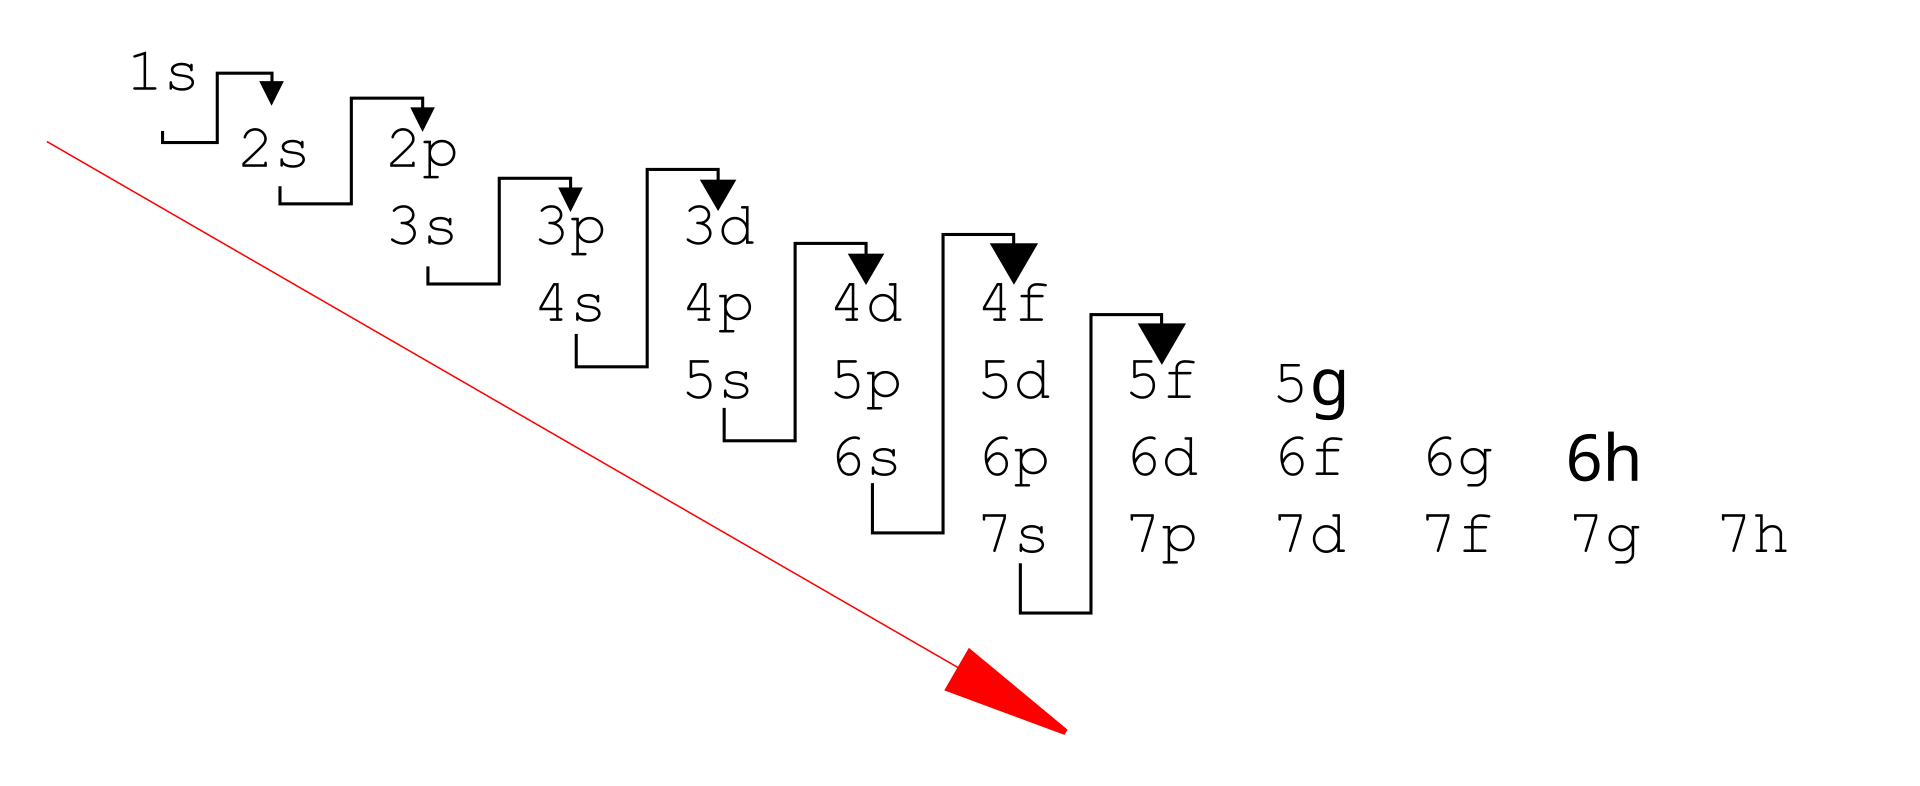
\includegraphics[scale=0.15]{./assets/klechkowski_rule.png}
\caption{Règle de Klechkowski}
\label{fig:klechkowski}
\end{center}
\end{figure}
\paragraph{Exceptions à la règle de l'Aufbau} Il existe certaines exceptions à ces règles \textbf{ELLES NE SONT PAS AU PROGRAMME}, mais il faut être au courant de leur existence.
\begin{figure}[h!]
\begin{center}
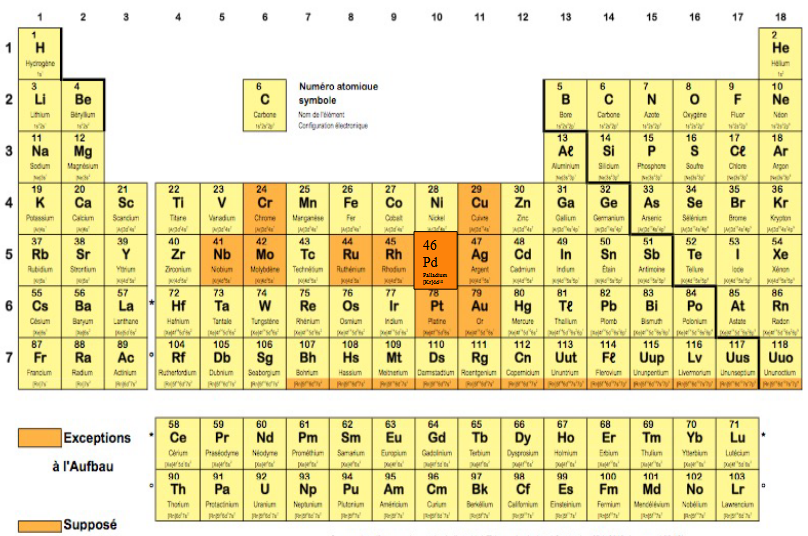
\includegraphics[scale=0.45]{./assets/aufbau_exceptions.png}
\end{center}
\caption{Exceptions à l'Aufbau}
\label{fig:exceptions}
\end{figure}
\newpage

\subsection{Classification périodique des éléments}

\paragraph{Classification selon Z} La classification des éléments se fait selon l'ordre croissant du numéro atomique \textbf{Z}. Les 92 premiers éléments sont dits "naturels" tandis que les éléments de 93 à 118 ont été préparés artificiellement. \par
Les colonnes sont désignées par un numéro de 1 à 18 ou par des symboles (IA, IIA, IIB...). Les éléments d'une même colonne constituent un groupe et portent un nom particuliers (i.e. métaux alcalins, gaz rares, halogènes, alcalino-terreux...). Ils ont également le \textbf{même nombre d'électrons de valence\footnote{électrons sur la dernière couche électronique de l'atome}}. \par 
Les lignes sont appelées \textbf{périodes}, elles sont numérotées de 1 à 7.
\paragraph{Le rayon atomique} Il existe plusieurs définitions du rayon atomique: par le calcul et la demi-distance entre centres d'atomes voisins (données expérimentales). \par
Le rayon atomique augmente en bas le long d'un groupe et diminue de gauche à droite le long d'une période ($Z_{eff}$\footnote{Zeff est la charge effective ressentie par l’électron le plus éloigné du noyau. Elle dépend de la charge du noyau et des autres électrons de l’atome.} $\nearrow$):
\begin{displaymath}
r \propto \frac{n^2}{Z_{eff}}
\end{displaymath}

\subsubsection{Charge nucléaire effective $Z_{eff}$}

\begin{displaymath}
Z_{eff} = Z - \delta
\end{displaymath}
avec $Z_{eff}$ la charge nucléaire effective, Z la charge nucléaire réelle et $\delta$ l'effet d'écran des électrons.
\begin{figure}[h!]
\begin{center}
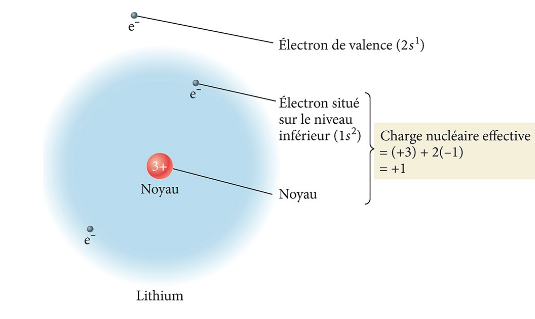
\includegraphics[scale=0.75]{./assets/zeff_example.png}
\end{center}
\caption{Exemple de $Z_{eff}$}
\label{fig:Zeff}
\end{figure}
\paragraph{L'énergie d'ionisation} Elle diminue de haut en bas d’un groupe et augmente le long d’une période.
\begin{displaymath}
IE = -E_n = \frac{Z_{eff}^2R_h}{n^2}
\end{displaymath}

\section{L'électronégativité}

\paragraph{Prédiction des propriétés des éléments} \hypertarget{electronegativity}{L'éléctronégativité} traduit le pouvoir \textbf{electro-attracteur} d'un atome lorsqu'il est engagé dans une liaison. \par 
Cette échelle arbitraire allant de 0 à 4 est sans unité. \\
L'électronégativité détermine le partage des électrons dans une liaison: les électrons vont se diriger vers l'atome le plus électronégatif.

\subsection{Récapitulatif des tendances périodiques}

\begin{figure}[h!]
\begin{center}
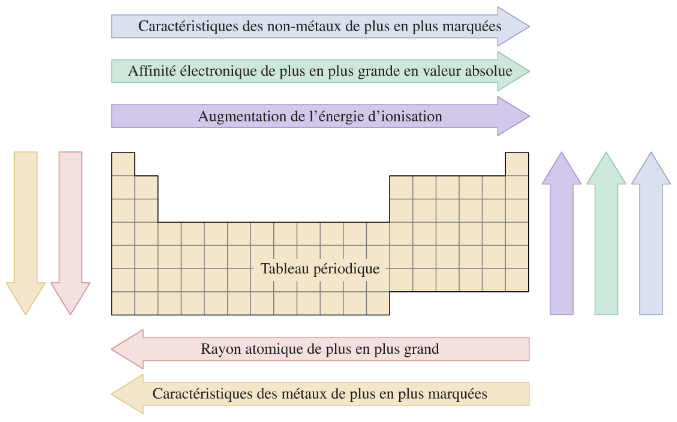
\includegraphics[scale=0.75]{./assets/recap_tendencies.png}
\end{center}
\caption{Récapitulatif des tendances périodiques}
\label{fig:recap}
\end{figure}

\chapter{Liaisons chimiques}

\section{Introduction}

\paragraph{Qu'est-ce qu'une liaison chimique ?} Une liaison chimique est un ensemble de forces électriques assurant la cohésion des molécules, elles résultent du partage du \textbf{partage d'électrons entre les atomes}. \par
Une liaison chimique correspond toujours à un \textbf{minimum énergétique}, elle se forme si l'arrangement des atomes final à une énergie \textit{plus faible} que la des énergies des atomes séparés. Par conséquent la formation de liaisons à pour conséquence \textbf{un dégagment d'énergie}.

\subsection{Les types de liaisons}

\paragraph{Liaison ionique} Une liaison entre \textbf{deux ions de signes \textit{opposés}} avec un passage d'électrons d'un atome à l'autre.\\ %need precisions 
\textbf{Cette liaison requiert une grande différence d'électronégativité !} ($\Delta$EN $>$ 1.7)
\paragraph{Liaison covalente} Cette liaison résulte d'un partage d'électron(s) entre deux atomes d'électronégativité semblable. Elles se distinguent entre les liaisons covalentes \textit{polaires} et \textit{apolaires}. \par
La force électroattractrice d'un atome est quantifié par son \hyperlink{electronegativity}{électronégativité}. Tant que $\Delta$EN $<$ 0.4 on parle de \textbf{liaison covalente non polaire} (ou covalente pure si $\Delta$EN = 0 comme pour $H_2$) , ensuite  entre 0.4 $<$ $\Delta$EN $<$ 1.7 on parle de \textbf{liaison covalente polaire} 
\paragraph{Liaison métallique} Il s'agit du partage des électrons de valence entre tous les atomes d'un métal (électronégativité faible), les électrons ainsi libres permettent la conductivité électrique !
\newpage

\section{Théorie de Lewis}

\paragraph{Les fondements de la théorie de Lewis} Selon Lewis les \textbf{électrons de valence} (électrons avec la valeur \textit{n} la plus grande) jouent un rôle fondamental dans les liaisons chimiques. \par
Lorsque les atomes perdent, recoivent ou partagent des électrons au cours de liaisons ils vont \textit{en général} acquérir la configuration électronique d'un \textbf{gaz noble}: ce sont les règles du \textbf{duet et de l'octet}\footnote{Seuls l'hydrogène (H), le lithium (Li) et le béryllium (Be) observent la règle du duet et prennent la forme de l'hélium (He)}.

\subsection{La représentation de Lewis}

La représentation de Lewis se concentre sur la couche externe que l'on représente simplifiée à l'aide de points symbolisant les \textbf{électrons de valence}. Les quatres premiers électrons sont représentés isolés, puis on groupe les électrons additionnels sous la forme de \textbf{doublets}.
% ajouter la partie sur les liaisons ioniques

\subsubsection{Méthodologie de Lewis (liaisons covalentes)}

\begin{enumerate}
\item Dénombrer les électrons de valence des tous les atomes de la molécule
\item Dessiner le \textbf{squelette} de la molécule en reliant les atomes les uns aux autres par une paire d'électrons. L'atome le \textbf{moins électronégatif} occupe la place \textbf{centrale}.
\item Placer les électrons restants sur l'atome central.
\item Si le nombre d'électrons disponibles est insuffisant il faut introduire des \textbf{liaisons multiples} et attribuer les charges de l'ion
\end{enumerate}
\textbf{Exemple: NH$_3$}
\begin{center}
\begin{enumerate}
\item \charge{0=\.,90=\:,180=\.,270=\.}{N}
\item \chemfig{\charge{90=\:}{N}(-[:0]H)(-[:180]H)(-[:270]H)}
\item Pas nécessaire ici.
\item Pas nécessaire ici.
\end{enumerate}
\end{center}
\textbf{Exemple: AsCl$_3$}
\begin{enumerate}
\item On dénombre le nombre d'électrons de valence:
\begin{itemize}
	\item 5 pour l'As
	\item 3$\times$7 pour Cl$_3$
\end{itemize}
\item On dessine le squelette et on relie: \chemfig{As(-[:45]Cl)(-[:135]Cl)(-[:270]Cl)}
\item On complète les octets (24 électrons utilisés) : \chemfig{As(-[:45]\charge{315=\|,45=\|,135=\|}{Cl})(-[:135]\charge{225=\|,45=\|,135=\|}{Cl})(-[:270]\charge{0=\|,180=\|,270=\|}{Cl})}
\item Placer les électrons restants sur l’atome central: \chemfig{\charge{90=\|}{As}(-[:0]\charge{0=\|,90=\|,270=\|}{Cl})(-[:180]\charge{90=\|,180=\|,270=\|}{Cl})(-[:270]\charge{0=\|,180=\|,270=\|}{Cl})}
\item %TODO add note
\end{enumerate}
\paragraph{Limites de la représentation de Lewis} Il s'agit d'une représentation empirique, cependant couplée à la représentation VSPR (voir \ref{VSPR}) elle permet une représentation géométrique de la forme de la molécule une estimation de sa polarité et de sa réactivité chimique. \\
Par exemple la règle de l’octet (ou doublet (H, He, Li, Be)) ne s’applique pas à tous les éléments/molécules !
\begin{itemize}
\item Hypovalence
\item Hypervalence
\item Les molécules à nombre impair d'électrons de valence (i.e. NO qui possède 11 électrons de valence)
\end{itemize}
De plus certaines propriétés comme le \textbf{paramagnétisme} doivent être décrites avec une représentation plus précise des électrons (la notion du spin voir \ref{spin}).

\section{Représentation VSEPR} \label{VSPR}

\subsection{Le modèle RPEV ou VSPER}

Le modèle de la Répulsion des Paires d’Electrons de Valence (RPEV) ou le Valence-Shell Electron-Pair Repulsion (VSEPR). \\
Lorsque l'on considère un atome, les paires d’électrons liantes et non liantes se placent de telle sorte à \textbf{minimiser} leur énergie de répulsion, la forme de la molécule dépend donc des atomes liés à \textbf{l'atome central}.
\begin{displaymath}
AX_nE_m
\end{displaymath}
A: atome central \\
n: nombre d’atomes liés à l’atome central \\
m : nombre de doublets libres de l’atome central \par
Les molécules de types AX$_n$E$_m$ ont une description \textbf{électronique} dépend des \textbf{atomes liés} et des \textbf{doublets non liants}. Cependant la \textbf{géométrie moléculaire} \textit{ignore} ces derniers.
\paragraph{Géométrie des molécules} On définit $\alpha_1$ et $\alpha_2$ les angles axiaux et équatoriaux des molécules\footnote{Pour des raisons de concision on se contentera ici de tableaux récapitulants les structures ;)}.
\begin{figure}[h!]
\begin{center}
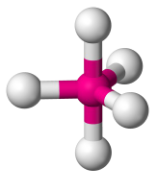
\includegraphics[scale=0.75]{./assets/geometry_example.png}
\caption{Example de géometrie avec $\alpha_1$ = 120° et $\alpha_2$ = 90°}
\label{fig:geometry_ex}
\end{center}
\end{figure}
\begin{figure}[h!]
\begin{center}
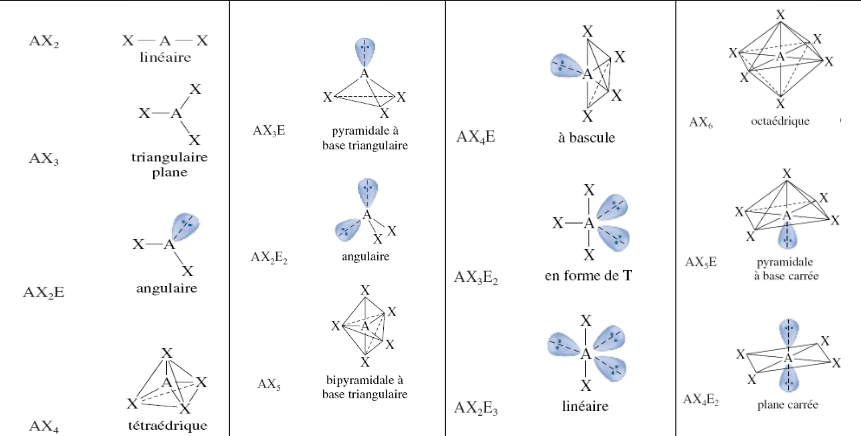
\includegraphics[scale=0.65]{./assets/geometry_table.png}
\caption{Tableau des géométries}
\label{fig:geometry_table}
\end{center}
\end{figure}
%TODO add the two other tables in a nicer way

\subsection{Polarité des molécules}

\title{Le moment dipolaire:}
\begin{displaymath}
\mu = \delta \times l
\end{displaymath}
$\delta$: charge électrique partielle résultant de la polarisation \\
$l$: longueur de la liaison\\
Par exemple pour HCl:\\
\begin{center}
$\delta+$ \; \; $\delta-$ \\
\chemfig{H(-[:0]Cl)}
\end{center}
Avec $\mu$ = 1,02D\footnote{1 D (Debye) = 3,36 x 10$^{-30}$ C$\cdot$m}
\paragraph{Géométrie et polarité} Les molécules dites \textbf{symétriques} son \textbf{apolaires} (la somme vectorielle des moments dipolaires est nulle) même si les liaisons individuelles sont polaires \\
À l'inverse les molécules dites \textbf{asymétriques} conduit (en cas de présence de liaisons individuelles polaires) à une molécule \textbf{polaire}.

\section{Approche quantique}

\subsection{Recouvrement des orbitales}

\paragraph{Théorie de la liaison de valence} Une liaison covalente résulte de la formation d’un doublet d’électrons de spins opposés dans la région du recouvrement de deux orbitales atomiques. \\
Exemple, formation d'H$_2$:
\begin{enumerate}
\item Deux atomes d’hydrogène se rapprochent l’un de l’autre. Ils renferment chacun un électron dans l’orbitale 1s de spin opposés.
\item A une certaine distance, les orbitales commencent à se chevaucher : recouvrement des orbitales 1s. \\
La région du recouvrement contient alors 2 électrons de spins opposés.
\item Augmentation de la densité électronique dans la région située entre les 2 noyaux : maintient ensemble les 2 noyaux.
\end{enumerate}

\subsection{Hybridation}

Exemple, le méthane CH$_4$:
\begin{center}
La configuration de C à l'état fondamental: \\ \vspace{0.5cm}
\begin{tabular}{| c | c | c | c | c |}
\hline
$\uparrow\downarrow$ & $\uparrow\downarrow$ & $\uparrow$ & $\uparrow$  & \: \\
\hline
\end{tabular}\\
1s \quad 2s \quad \qquad 2p
\end{center}
\par On constate que l'orbitale 2p contient deux électrons non appariés $\rightarrow$ on prédit alors que la molécule la plus simple est CH$_2$. Cependant CH$_2$ n'est pas stable, l'hydrocarbure stable le plus simple est CH$_4$. \par
Cependant pour construire CH$_4$ on a besoin de 4 électrons non appariés. Il faut donc:
\begin{enumerate}
\item Promouvoir des électrons dans les orbitales d'énergie supérieure.
\item Il faut que les quatre orbitales de l’atome de C qui vont se recouvrir avec l’orbitale 1s des atomes d’hydrogène soient identiques.
\end{enumerate}
C'est \textbf{l'hybridation} des orbitales \textbf{2s} et \textbf{2p} $\rightarrow$ 4 orbitales équivalentes quant à la forme et l'énergie.
\paragraph{L'hybridation ne se limite pas au carbone} %TODO ajouter le reste de l'hybridation (?)
\paragraph{L'hybridation des atomes dans une molécule complexe:}
\begin{itemize}
\item le nombre d’orbitales hybrides d’un atome donné est la somme des atomes liés et des doublets non liants d’électrons.
\item Les atomes terminaux liés par une seule liaison ne sont pas hybridés.
\end{itemize}
\begin{figure}[h!]
\begin{center}
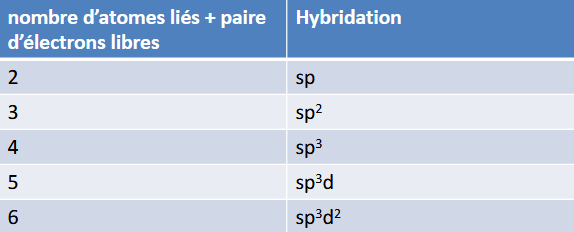
\includegraphics[scale=0.65]{./assets/hybridation_table.png}
\caption{Tableau des hybridations}
\label{fig:hybridation_table}
\end{center}
\end{figure}

\subsection{Liaisons $\delta/\pi$ et hydrogène}

\subsubsection{Les liaisons $\delta$}

\begin{itemize}
\item Symétrie cylindrique autour de l’axe de liaison.
\item Liaison formée par recouvrement axial.
\item Il s'agit d'une liaison \textbf{très stable}.
\item Les deux atomes liés peuvent tourner autour de l’axe de la liaison.
\end{itemize}

\subsubsection{Les liaisons $\pi$}

\begin{itemize}
\item Axe de liaison dans un plan nodal.
\item Liaison plus \textbf{faible} que la liaison $\delta$
\item Les deux atomes liés ne peuvent pas tourner autour de l’axe de la liaison.
\end{itemize}

\subsubsection{Les liaisons hydrogène}

Une liaison hydrogène est formée par un atome d’hydrogène placé entre deux atomes très électronégatifs. Seuls les atomes F, O et N sont suffisamment petits et électronégatifs pour
qu’une telle liaison se forme.
\begin{itemize}
\item L’atome d’hydrogène (1 seul électron) est lié avec un atome très électronégatif (charges
partielles considérables).
\item Un atome avec au moins une paire d’électrons se lie à l’atome d’hydrogène.
\item Les atomes sont assez petits et peuvent être très proches.
\end{itemize}

\chapter{Stoechiométrie}

\section{Quantités chimiques}

\subsection{Quantité de matière / microscopique}

\subsubsection{Masse atomique}

L'unité de masse atomique (u.m.a.) équivaut à $ \frac{1}{12} $ème de la masse d'un atome $^{12}$C. \\ 
1 u.m.a. = 1 Da\footnote{Da: \href{https://fr.wikipedia.org/wiki/Unit\%C3\%A9_de_masse_atomique_unifi\%C3\%A9e\#En_biochimie}{le Dalton} \label{fn:3}} = 1,66054 $\times$ 10$^{-24}$g \\
La masse atomique d’un élément tient compte de l’abondance naturelle des différents isotopes et peut être considérée comme une donnée expérimentale affichée sur le tableau périodique.\\
Exemple: masse atomique l'oxygène \\
15,9994 u.m.a. = 15,9994 $\times$ 1,66054 $\times$ 10$^{-24}$ g = 2,65676 $\times$ 10$^{-24}$ g

\subsubsection{Masse moléculaire}

La somme des masses de chacun des atomes constituant une molécule. Elle est aussi donnée en uma ou Da.\footnote{Le défaut de masse est négligeable dans une liaison chimique}\\
Exemple: masse moléculaire de H$_2$O \\
(2 $\times$ 1,0079) + (1 $\times$ 15,9994) = 18,0152 Da$^{\ref{fn:3}}$ = 2,99 $\times$ 10$^{-23}$g

\subsubsection{La mole}

Unité qui permet de rapporter simplement les nombres gigantesques d’atomes et de molécules dans des échantillons visibles.
\paragraph{Définitions} 1 mole d’atomes = quantité de substance contenant le même nombre d’atomes que 12 g de $^{12}$C pur. \par
Ce nombre c'est \textbf{le nombre d'Avogadro} ($N_A$) = 6,022 $\times$ 10$^{23}$ mol$^{-1}$
\begin{itemize}
\item 1 atome de $^{12}$C pèse 12 Da (12 u.m.a.)
\item 1 mol d’atomes de $^{12}$C pèse 12 g
\item Donc pour 1 mol de $^{12}$C, on peut écrire 1 mol $\times$ $N_A$ $\times$ 12 Da = 12 g
\item Soit $N_A$ = 1 g$\cdot$Da$^{-1}$ $\cdot$mol$^{-1}$ \footnote{Nouvelle définition IUPAC 2018: La mole est l’unité de quantité de matière qui contient 6.02214076 $\times$ 10$^{23}$ particules élémentaires} \\
\end{itemize}

\subsection{Quantité de matière / macroscopique}

\subsubsection{Masse molaire d’un composé ou d’un élément}

Masse d’une mole de molécules (atomes, ions etc.) donnée en g/mol. \\
On la calcule ainsi à partir des données du tableau périodique:
\begin{displaymath}
M = {\sum_i}M_i(E_i){\times}n_i
\end{displaymath}
La masse molaire est la somme de la masse atomique $M_i$ de chaque élément $E_i$ qui compose la molécule, multipliée par le nombre $n_i$ d’atomes de cet élément présent dans la molécule. \\
Exemples:
\begin{itemize}
\item Masse molaire de $^{12}$C = 12 Da . $N_A$ = 12 $\times$ 1,66 $\times$ 10$^{-24}$ g $\times$ 6,022 $\times$ 10$^{23}$ mol$^{-1}$ = 12 g$\cdot$mol$^{-1}$\footnote{On remarque que la masse molaire en g mol-1 a la même valeur numérique que la masse moléculaire en u.m.a. ou Da}
\item Masse molaire : H$_2$O (2 $\times$ 1,0079) + (1 $\times$ 15.9994) g = 18,0152 g$\cdot$mol$^{-1}$
\end{itemize}

\subsubsection{Unités de concentrations pour solutions}

\begin{center}
\begin{tabular}{| c | c | c |}
\hline
\textbf{Concentration} & \textbf{Unités} & \textbf{Définition} \\
\hline
Molarité M  & mol$\cdot$L$^{-1}$ & atm\\
\hline
Molalité m  & mol$\cdot$kg$^{-1}$ & bar \\
\hline
Fraction molaire $\chi$  &  & $\frac{n_{solute}}{n_{solute}+n_{solvant}} $\\
\hline
\% volumique  &   & $\frac{V_{solute}}{V_{solution}\times100}$\\
\hline
\% masse &  & $\frac{m_{solute}}{m_{solution}\times100}$ \\
\hline
\end{tabular}
\end{center}

\subsection{Théorie cinétique des gaz}

\paragraph{Définition} Un gaz est un ensemble de particules en mouvement constant. e mouvement est rectiligne et les collisions avec les parois ou d’autres molécules est parfaitement élastique (pas de perte d’énergie globale). \\
L’énergie cinétique moyenne d’une molécule est proportionnelle à la température. \\
La taille des particules de gaz est négligeable par rapport au volume dans lequel, elles évoluent. \\
\begin{displaymath}
\tag*{\textbf{Constante des gaz parfaits}}
PV = nRT \label{eq:PVNRT}
\end{displaymath}\\
\begin{center}
\begin{tabular}{| c | c | c | c | c |}
\hline
\textbf{R} & \textbf{V} & \textbf{P} & \textbf{T}  & \textbf{n} \\
\hline
0.0821 L$\cdot$atm$\cdot$K$^{-1}\cdot$mol$^{-1}$  & L & atm & K  & mol \\
\hline
0.0831 L$\cdot$bar$\cdot$K$^{-1}\cdot$mol$^{-1}$  & L & bar & K  & mol \\
\hline
0.0821 L$\cdot$kPa$\cdot$K$^{-1}\cdot$mol$^{-1}$  & L & kPa & K  & mol \\
\hline
8.314 L$\cdot$K$^{-1}\cdot$mol$^{-1}$  & m$^3$ & Pa & K  & mol \\
\hline
\end{tabular}
\end{center}

\subsubsection{Conditions standard} \label{condStands}
\begin{itemize}
\item P = 1 bar = 100 kPa\footnote{Anciennement on utilisait P =1 atm (dont l’usage n’a pas complètement disparu)}
\item La température n'est pas une condition standard à proprement parler, cependant on choisit en général 25°C (298K\footnote{K = T$_{ °C}$ + 273,15})
\end{itemize}

\subsubsection{Conditions normales (TPN)}\footnote{Dans ces conditions \textbf{une mole de gaz} occupe un volume de \textbf{22,4 L}}

\begin{itemize}
\item P = 1 atm = 101, 325 kPa
\item T = 273,15 K (0°C)
\end{itemize}

\subsubsection{Pression partielle d'un gaz}

La pression partielle d’une espèce i, Pi, dans un mélange est la contribution de la seule
espèce i à la pression totale.
\begin{center}
\title{Loi de Dalton\footnote{Ne s'applique qu'aux gaz parfaits.}}
\end{center}
\begin{displaymath}
P_i = x_i \times P_{tot}
\end{displaymath}

\begin{itemize}
\item $P_i$ la pression partielle de l'espèce i
\item $x_i$ est la fraction molaire de l’espèce i\footnote{nombre de mol de l’espèce i/nombre de mol total des espèces présentes ($\frac{n_i}{n_{tot}}$)}
\item $P_{tot}$ la pression totale du mélange
\end{itemize}
\newpage

\section{Équation chimique} 

\begin{displaymath}
R\acute{e}actifs \longrightarrow Produits
\end{displaymath}
\paragraph{Propriétés} Lors d'une réaction chimique il y a \textbf{conservation} du nombre de chacun des atomes et \textbf{conservation} de la charge électrique totale. \\
Les lettres indiquent des états/informations supplémentaires:
\begin{itemize}
\item A(g) phase gazeuse
\item A(l) phase liquide
\item A(s) phase solide
\item A(sol) solution
\item A(aq) solution aqueuse
\end{itemize}
\begin{displaymath}
C_2H_5OH(l) + 3\footnote{3 est ici un \textbf{coefficient stoechiométrique}}O_2(g) \rightarrow 2CO_2 (g) + 3H_2O(l)
\end{displaymath}
Exemple:
On constate qu'il y a exactement le même nombre d'atomes des deux côtés\footnote{2 atomes de C, 6 d'H, 7 d'O} la réaction est \textbf{équilibrée}.

\subsection{Classification des réactions}

\paragraph{Cas d'équilibre} Il s'agit du cas général défini par la thermodynamique. La réaction peut evoluer dans les deux sens.
\begin{displaymath}
N_2(g) + 3H_2(g) \rightleftarrows 2NH_3(g)
\end{displaymath}
\paragraph{Réaction complète} Celle-ci a lieu lorsque l'équilibre est déplacé artificiellement.
\begin{displaymath}
CaCO_3(s) \xrightarrow{\Delta} CaCO(s) + CO_2(g)
\end{displaymath}
Ici $\Delta$ est le \textbf{chauffage} de la réaction qui cause le déplacement de l'équilibre.
\paragraph{Réaction acide-base} Réaction basée sur le transfert de protons entre un couple acide/base.
\paragraph{Réaction d'oxydo-réduction} Réaction basée sur le transfer d'électrons entre un couple oxydant/réducteur
\paragraph{Et bien d'autres} On retrouve aussi des réactions dites de complexation, de substitution, de dissociation ou de précipitation.

\subsubsection{Cas particulier: réaction de précipitation}

\textbf{Équation moléculaire globale:}
\begin{displaymath}
2KI(aq) + Pb(NO_3)_2(aq) \longrightarrow 2KNO_3(aq) + PbI_2(s)
\end{displaymath}
\textbf{Équation ionique complète:}
\begin{displaymath}
2K^+(aq) + 2I^-(aq) + Pb^{2+}(aq) + 2NO_3^-(aq) \longrightarrow 2K^+ (aq) + 2 NO_3^-(aq) + PbI_2(s)
\end{displaymath}
On constate que $K^+$ et $NO_3^-$ ne participent pas à la réaction de précipitation mais sont présents dans la solution. Ils sont \textbf{ions spectateurs}. \vspace{0.2cm} \\
\textbf{Équation ionique nette (sans ions spectateurs) :}
\begin{displaymath}
2I^-(aq) + Pb^{2+}(aq) \longrightarrow PbI_2(s)
\end{displaymath}

\subsection{Stoechiométrie}

\paragraph{Loi de conservation de masse} Au cours d’une réaction chimique, on peut considérer que la masse est conservée\footnote{Sauf en cas de réaction nucléaire. Ce qui est en réalité conservé c’est la masse-énergie.}. \par
Interprétation de Dalton : au cours d’une réaction chimique, les atomes ne sont ni créés ni détruits, ils changent de partenaires. \par
Les \textbf{coefficients stoechiométriques} sont introduits pour \textbf{équilibrer} les réactions: ils permettent d'avoir le même nombre d'atomes de chaque côté de la flèche.\\
Exemple: la combustion du butane (C$_4$H$_10$)
\begin{displaymath}
2C_4H_10(g) + 13O_2(g) \longrightarrow 8CO_2(g) + 10H_2O(l)
\end{displaymath}
En mole on a: 2 + 13 $\longrightarrow$ 8 + 10
En masse: 2 $\times$ 58 + 13 \x 32 $\longrightarrow$ 8 \x 44 + 10 \x 18

\subsubsection{Réactif limitant}

Le réactif \textbf{limitant} n'apparaît qu'en dehors des conditions stoechiométriques, il est celui qui détermine la \textbf{quantité maximale de produit} qui peut être formée. \\
Il est celui qui disparaît complètement à l'avancement x$_{max}$. \\
Exemple: La combustion du propane
\begin{displaymath}
C_3H_8(g) + 5O_2(g) \longrightarrow 3CO_2(g) + 4H_2O(l)
\end{displaymath}
\begin{itemize}
\item La flèche unique vers la droite indique que la réaction inverse n'a \textbf{pas} lieu.
\item Le rapport molaire optimal pour les réactifs est 1:5 et le rapport des produits est 3:4.
\item Dans le cas ou l'apport de réactif ne respecterait pas le rapport 1:5 pour le C$_3$H$_8$ et l'O$_2$ alors il resterait de \textbf{l'un des deux} réactifs.
\item Exemple: pour 1 moles d'C$_3$H$_8$ et 7,5 moles d'O$_2$ on obtient 3 moles de CO$_2$ et 4 moles d'H$_2$O ET un reste de 2,5 moles d'O$_2$.
\end{itemize}

\subsubsection{Rendement $\eta$}

Le rendement exprime le pourcentage de complétion réel de la réaction par rapport au pourcentage de complétion théorique.
\begin{displaymath}
A \longrightarrow B
\end{displaymath}
\begin{displaymath}
\eta_s = \frac{masse \: de \: B \: pratique}{masse \: de \: B \: th\acute{e}orique} \times 100 = \frac{mole \: de \: B \: pratique}{mole \: de \: B \: th\acute{e}orique} \times 100
\\
\end{displaymath}
$\eta$ < 100\% dans les cas suivants:
\begin{itemize}
\item Réactions incomplètes (réversibles) A $\rightleftarrows$ B
\item Formation de produits secondaires A $\rightarrow$ B + C
\end{itemize}

\section{Réactions rédox}

\subsection{Introduction}

Les équations \textbf{d'oxydo-réduction} sont des réactions avec \textbf{transfert d'électrons}. Il faut donc faire attention à la conservation de la \textbf{masse} et de \textbf{la charge globale}. \\
Exemple: 
\begin{displaymath}
\textbf{2}Ag^+(aq) + Cu(s) \longrightarrow \textbf{2}Ag(s) + Cu^{2+}(aq) 
\end{displaymath}
On aurait pu avoir seulement:
\begin{displaymath}
Ag^+(aq) + Cu(s) \longrightarrow Ag(s) + Cu^{2+}(aq) 
\end{displaymath}
La masse serait alors bien conservée mais pas la charge globale: la réaction n'est pas complètement équilibrée. \par
Au niveau moléculaire la réaction qui a lieu est un \textbf{transfer d'électrons} allant de Cu (donneur d'électrons, \textbf{réducteur}) à Ag$^+$ (accepteur d'électrons, \textbf{oxydant}). \par
Comme Cu libère deux électrons il nous faut deux cations Ag$^+$ prêts à les recevoir. Il faut que \textbf{le nombre d'électrons donnés par le réducteur soit égal au nombre d'électrons acceptés par l'oxydant}.

\subsection{Degré d'oxydation}

Le degré d'oxydation (d.o) indique le nombre d'électrons que chaque atome aurait donné ou reçu par rapport à l'état neutre si les liaisons dans lesquelles ces atomes sont impliqués étaient de nature purement ionique. \par 
Si l'électronégativité des deux atomes liés est la même (par exemple, si les atomes liés sont un même élément), alors la liaison \textbf{ne contribue pas} au calcul du d.o. \\
Exemples: 
\begin{displaymath}
\chemfig{O^{-2}(-[:0]H^{+1})(-[:180]H^{+1})}
\end{displaymath}
\begin{displaymath}
\chemfig{H^{+1}-O^{-1}-O^{-1}-H^{+1}}
\end{displaymath}
\begin{displaymath}
\chemfig{O^{+2}=C^{-4}=O^{+2}}
\end{displaymath}
Comme chaque liaison est considérée comme \textbf{ionique} on "transfère" pour chaque liaison les électrons vers l'atome le plus électronégatif de la liaison.
\paragraph{Règles définissant le degré d'oxydation}
\begin{itemize}
\item Le \textbf{fluor (F)} a \underline{toujours} un d.o. égal à \textbf{-1}.
\item Les \textbf{métaux alcalins} (Li, Na, etc.) ont \underline{toujours} un d.o. égal à \textbf{+1}.
\item Les \textbf{métaux alcalino-terreux} (Be, Mg, etc.) ont \underline{toujours} un d.o. égal à \textbf{+2}.
\item \textbf{L'hydrogène} possède \textit{en général} un d.o. égal à \textbf{+1}\footnote{À l’exception des hydrures de métaux où il a un d.o. de -1.}.
\item \textbf{L'oxygène} a \textit{en général} un d.o. égal à \textbf{–2}\footnote{Sauf s’il est lié avec lui-même ou avec du fluor.}.
\end{itemize} \par
Dans une espèce chimique neutre (molécule ou radical), la somme des d.o. des atomes est nulle. En revanche si le composé est chargé, cette somme est égale à la charge de l’ion\footnote{Dans ce cours, nous nous restreignons aux composés dont
le degré d’oxydation vaut +1 pour H et -2 pour O. Dans un élément comme H2 ou
O2, le degré d’oxydation vaut 0}.

\subsection{Équilibrage d'une équation d'oxydo-réduction}

\begin{enumerate}
\item Repérer les éléments dont le degré d’oxydation (D.O.) change au cours de la réaction.
\item Le nombre d’électrons cédés par le réducteur doit être égal au nombre d’électrons acquis par l’oxydant; ceci permet de trouver quatre coefficients.
\item S’il figure dans l’équation d’autres substances dont le D.O. n’est pas affecté, il faut
trouver le coefficient de ces substances par un bilan des masses.
\item Si des réactifs et/ou des produits sont des ions, il faudra vérifier le calcul par un
bilan des charges.
\end{enumerate}
Exemple: 
\begin{displaymath}
HBr + KClO_3 \longrightarrow Br_2 + H_2O + KCl
\end{displaymath}
\begin{enumerate}
\item Élements dont le d.o. change: Br (-1 $\xrightarrow{-1e}$ 0), Cl (+5 $\xrightarrow{+6e}$ -1) 
\item
\begin{displaymath}
HBr^{-1} + KClO_3^{+5} \longrightarrow Br_2^{+0} + H_2O + KCl^{-1} 
\end{displaymath}
\item Donc on a 6 \x -1e du HBr pour équilibrer le 1 \x +6e KCl (on équilibre le reste selon les masses).
\begin{displaymath}
\textbf{6}HBr + \textbf{1}KClO_3 \longrightarrow \textbf{3}Br_2 + \textbf{3}H_2O + \textbf{1}KCl
\end{displaymath}
\end{enumerate}
%TODO add le second exemple (la flemme de tout copier maintenant

\chapter{Thermodynamique}

\section{Introduction}

\paragraph{Particularités} En chimie on  considère un nombre réduit de fonctions et on s'intéresse à leurs variations lors d'une réaction chimique. On se placera dans des conditions standards (voir \ref{condStands}). Ces fonctions sont des variables d'état, leur valeur ne dépend pas du chemin parcouru mais uniquement de l'état initial et final du système.
\paragraph{Système, environnement, univers} Le \textbf{système} est le milieu réactionnel (en chimie. \textbf{L'environnement} est tout ce qui se trouve à l'extérieur du système. \textbf{L'univers} c'est l'ensemble système et environnement. \par 
Il existe différents types de systèmes: 
\begin{enumerate}
\item \textbf{Ouvert} : peut échanger énergie et matière.
\item \textbf{Fermé} : peut échanger de l'énergie  mais pas de matière.
\item \textbf{Isolé} : ne peut échanger ni matière, ni énergie.
\end{enumerate}

\section{Premier principe de la thermodynamique}

\par Durant une transformation, la variation d’énergie interne du système est égale
à la somme de la quantité de chaleur échangée avec l’environnement
et du travail fourni.
\begin{displaymath}
\Delta U = W + Q
\end{displaymath}
\begin{itemize}
\item $\Delta$U: variation d'énergie interne du système.
\item W: énergie fournie \textbf{au système} sous forme de \textbf{travail}.
\item Q: énergie fournie au système sous forme de chaleur (transfert d’énergie sous forme d’agitation de molécules)
\end{itemize}
\textbf{L'énergie est en tout cas conservée. Elle ne peut être ni créée ni détruite.}\footnote{Par convention L’énergie (sous forme de travail ou de chaleur) fournie au système est dénotée positivement}

\subsection{Énergie interne U et Enthalpie H}

Les réactions chimiques sont étudiées plutôt à pression constante (voir \ref{condStands}).
À pression constante, un travail \textbf{W = -P \x $\Delta$V} est fourni/perdu par le système\footnote{Ce travail est compté négativement lorsque le volume augmente d’où le signe négatif}.
\paragraph{Définition de l'enthalpie} 
\begin{displaymath}
H = U + PV
\end{displaymath}
\begin{displaymath}
\Delta H = \Delta U + P\footnote{pour $\Delta$P = 0 P$_{ext}$=P$_{sys}$=P}\Delta V
\end{displaymath}
\begin{displaymath}
\Delta H = W + Q + P\Delta V
\end{displaymath}
\begin{displaymath}
\Delta H = -P\Delta V + Q + P\Delta V
\end{displaymath}
\begin{displaymath}
\Delta H = Q_P
\end{displaymath}
La variation d’enthalpie du système DH est égale à la chaleur Q$_P$ fournie au système, à \underline{pression constante}.
\paragraph{Processus exothermique} Est un processus qui \textbf{libère} de la chaleur, à pression constante un processus exothermique a: $\Delta_r$H $<$ 0
\paragraph{Processus endothermique} Est un processus qui \textbf{absorbe} de la chaleur, à pression constante un processus exothermique a: $\Delta_r$H $>$ 

\subsubsection{Enthalpie des changements d'état}

\begin{figure}[h!]
\begin{center}
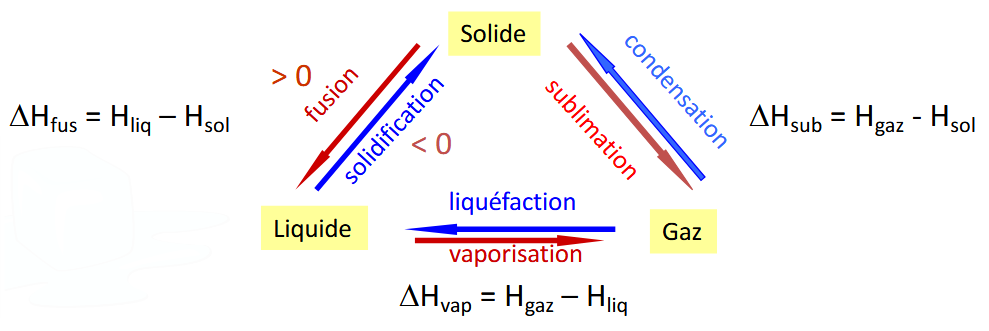
\includegraphics[scale=0.55]{./assets/enthalpy_states.png}
\caption{Enthalpie des changements d'état}
\label{fig:changements}
\end{center}
\end{figure}

\subsection{Calcul de l'enthalpie}

Il faut mesurer dans des conditions standardisées (1 mol de substance pure à des conditions de références \ref{condStands}): $\Delta_r$H$^0$

\subsubsection{Méthode 1: Enthalpie standard de formation $\Delta_f$H$^0$ (kJ/mol)}

L’enthalpie standard de formation d’un composé est la variation d’enthalpie de la réaction de formation d’une mole de composé à partir des éléments dans leur état de référence\footnote{Voir \ref{condStands} (again).}.
\begin{displaymath}
A + B + C \longrightarrow substance(ABC) \;\;\; \Delta_r H^0 \equiv \Delta_f H^0 (formation)
\end{displaymath}
$\Delta_f$H$^0$ est nulle pour la formation de tous les éléments dans leur état de référence.
\paragraph{Mesure de l'enthalpie de formation de CO$_2$(g)} On fait la réaction suivante dans un calorimètre: formation de 1 mol CO2 (g) à partir des éléments (ici C et O dans leur état de référence).
\begin{displaymath}
C (graphite, s) + O_2(g) \rightarrow CO_2(g)
\end{displaymath}
\begin{itemize}
\item $\Delta_r$H$^0$ = $\Delta_f$H$^0$ (CO$_2$) = -393,5 kJ$\cdot$mol$^-1$
\item $\Delta_f$H$^0$ (C, graphite) = $\Delta_f$H$^0$ (O$_2$, g) = 0 (par définition)
\end{itemize}
Dans ce cas, la pression externe reste égale à 1 bar pendant toute la réaction. Le volume ne change pas mais la température de l’environnement (et du système) augmente pendant la réaction exothermique. 
Cette variation de température est mesurée dans un calorimètre à pression constante
et reliée à l’enthalpie selon la relation $\Delta_r$H$^0$ = C$_p$ $\Delta$T
\paragraph{Enthalpies molaires standards de formation (conditions \ref{condStands})} \label{standard_formation_enthalpy}
\begin{center}
\begin{tabular}{| c | c |}
\hline
\textbf{Composé chimique} & \textbf{(kJ/mole)} \\
\hline
CO$_2$(g) & -393,5 \\
\hline
NH$_3$(g) & -46,1 \\
\hline
CH$_4$(g) & -74,6 \\
\hline
C$_2$H$_6$(g) & -84,7 \\
\hline
C$_3$H$_8$(g) & -103,88 \\
\hline
C$_4$H$_{10}$(g) & -126,2 \\
\hline
H(g) & 218 \\
\hline
O(g) & 249,28 \\
\hline
O$_2$(g) & 0 \\
\hline
C (graphite) & 0 \\
\hline
C (diamant) & 1,92 \\
\hline
H$_2$O (liquide) & -285,8 \\
\hline
H$_2$O (gaz) & -241,8 \\
\hline
\end{tabular}
\end{center}
\paragraph{L'enthalpie standard (molaire) de réaction $\Delta_r$H$^0$}
\begin{displaymath}
\Delta_r H^O = \sum^p_{i=1}v_i\Delta_f H_i^O \; (produits) \; - \; \sum^r_{j=1}v_j\Delta_f H_j^O \; (r\acute{e}actifs)
\end{displaymath}

\subsubsection{Méthode 2: Loi de Hess}

$\Delta$H$^0$ : l’enthalpie est une variable d’état et ne dépend que des états initial (i) et final (f). \par
Donc le changement d’enthalpie d’une réaction est toujours le même, que la réaction se produise en une ou plusieurs étapes.
\begin{displaymath}
\Delta_r H^0 = \Delta H_1^0 + \Delta H_2^0 + \Delta H_3^0 +...
\end{displaymath} \par
Si la réaction peut être découpée en trois étapes, l’enthalpie
de la réaction globale est la somme des enthalpies de réaction
de ces trois étapes. \par
Ces étapes n’ont pas nécessairement besoin d’être réalisables
au laboratoire. \\
On note aussi:
\begin{displaymath}
\Delta H \; (r\acute{e}action \: directe) \; = \; - \Delta H \; (r\acute{e}action \: inverse)
\end{displaymath}
%TODO ajouter un exemple maybe

\subsubsection{Méthode 3: Calcul de $\Delta_r$H$^0$ à partir des enthalpies de liaisons}

Cette méthode est considérée très simple mais moins précise. 
\begin{displaymath}
\Delta H^0_r = \sum H_L \; (r\acute{e}actifs) \; - \; \sum H_L \; (produits)
\end{displaymath}
Exemple:
\begin{displaymath}
2C(s) + H_2(g) \longrightarrow C_2H_2(g)
\end{displaymath}
Pour créer du C$_2$H$_2$ à partir du C(s) et H$_2$(g) il faut:
\begin{itemize}
\item Vaporiser deux moles C(s) -$>$ C(g): +2 \x 717 kJ/mol).
\item Casser une liaison H-H: +436 kJ/mol.
\item Former une triple liaison CXC: -812 kJ/mol.
\item Former deux liaisons C-H: 2 \x -414)kJ/mol.
\end{itemize}
Donc, on obtient \textbf{$\Delta_r$H$^0$} = 230 kJ/mol\footnote{REMARQUE: différence entre la somme des énergies des liaisons à rompre (réactifs) – somme des énergies des liaisons à faire (produits).}.
\begin{figure}[h!]
\begin{center}
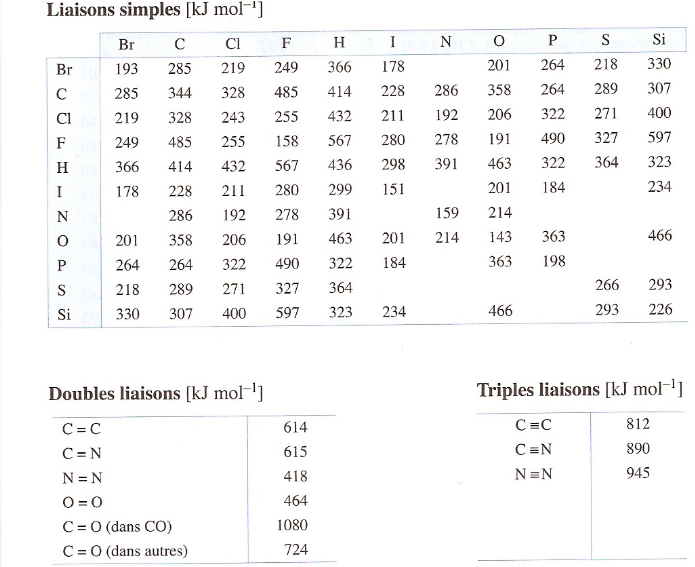
\includegraphics[scale=0.75]{./assets/enthalpy_links.png}
\caption{Enthalpie des liaisons}
\label{fig:enthalpy_links}
\end{center}
\end{figure}
\newpage

\subsection{Définitions de l’entropie}

Pour un système dans lequel une quantité de chaleur Q est échangée de manière réversible, à la température T :
\begin{displaymath}
\Delta S = \frac{Q_{rev}}{T}
\end{displaymath}
%TODO add some more text about it
\subsection{Limitations}

Le premier principe ne permet pas de déterminer la direction d’une réaction chimique: les \textbf{critères de spontanéité}. D’après le premier principe, la quantité d’énergie disparue sous une forme est égale à la quantité d’énergie qui apparaît sous une autre forme : ne s’oppose pas au retour à l’état initial. \par
Pour un gaz parfait, U ne dépend que de la température: $\Delta$U = 0 ($\Delta$H=0). \\
Processus \textbf{spontané} : a tendance à se produire sans influence extérieure. \\
Processus \textbf{non spontané} : ne se produit que s’il est provoqué.

\section{Deuxième principe de la thermodynamique}

Une transformation spontanée s’accompagne d’une augmentation totale de l’entropie de l’univers (système + environnement).
\begin{displaymath}
\Delta S_{uni} = \Delta S_{syst} + \Delta S_{env}  
\end{displaymath}
Si $\Delta$S$_{uni}$ $>$ 0 la réaction est \textbf{spontanée}. Dans le cas où $\Delta$S$_{uni}$ = 0 elle est réversible (équilibre). \par
On peut augmenter l'entropie d'une substance par \textbf{chauffage} qui cause augmentation du mouvement des molécules donc augmentation du désordre relatif des molécules, ou par \textbf{espace}, fournir plus d’espace pour disperser les molécules. \\
L’entropie d’une substance pure, parfaitement cristalline est nulle à zéro K. S = k ln W = 0 lorsque W = 1 (3ème principe). %TODO chercher ce que ça veut dire

\subsection{Entropie standard de réaction $\Delta_r$S$^O$}

\begin{displaymath}
R\acute{e}actifs \; (R) \; \longrightarrow \; Produits \; (P)
\end{displaymath}
\begin{displaymath}
\Delta_r S^0 = \sum n_P(S^0)_P - \sum n_R(S^0)_R 
\end{displaymath}
\begin{itemize}
\item S$^0$: entropie molaire standard (J$\cdot$K$^{-1}\cdot$mol$^{-1}$).
\item n: coefficient stoechiométrique (sans unité).
\end{itemize}
\begin{figure}[h!]
\begin{center}
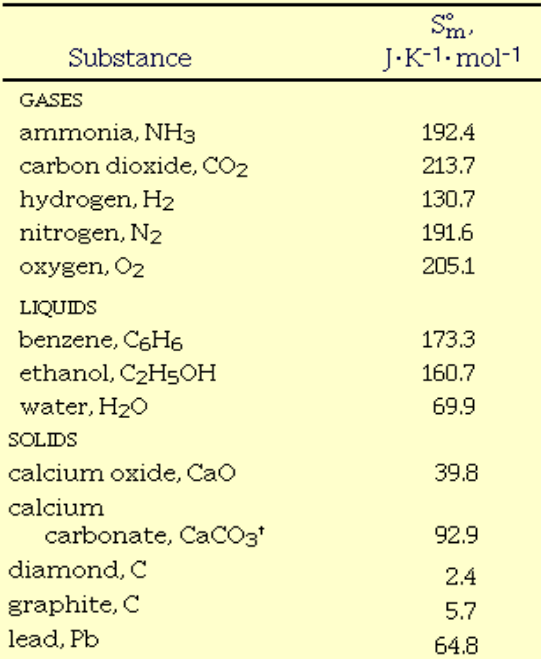
\includegraphics[scale=0.75]{./assets/enthropy_standards.png}
\caption{Enthropie molaire standard}
\label{fig:enthropy_molar}
\end{center}
\end{figure}

\paragraph{Exemple en conditions standards}\footnote{\ref{condStands}}
\begin{displaymath}
H_2(g) + \frac{1}{2}O_2(g) \longrightarrow H_2O(l)
\end{displaymath}
\begin{displaymath}
\Delta_r S^0 = S^0(H_2O(l)) - S^0(H_2(g)) - \frac{1}{2}S^0(O_2(g)
\end{displaymath}
\begin{displaymath}
\Rightarrow 69,9 - 130,7 - \frac{1}{2}(205,1) = -163,3J\cdot K^{-1}\cdot mol^{-1}
\end{displaymath} \par
Il est important de  noter que \textbf{S0(gaz) $\gg$ S0(liquides, solides)}. Ceci signifie que dans une réaction, une variation du nombre de moles gazeuses prédomine, en général, sur toute autre variation d’entropie.

\newpage

\subsection{Prédiction de la spontanéité d’une réaction}

On reprend l'exemple précédent: 
\begin{displaymath}
H_2(g) + \frac{1}{2}O_2(g) \longrightarrow H_2O(l)
\end{displaymath}
On a calculé \(\Delta_r S^0 = -163,3J\cdot K^{-1}\cdot mol^{-1}\) et on a \(\Delta_r H^0 = -285,8kJ\cdot mol^{-1}\) d'après les enthalpies standards de formation (voir \ref{standard_formation_enthalpy}).\\
On reprend:
\begin{displaymath}
\Delta S_{uni} = \Delta S_{syst} + \Delta S_{env} = \Delta_r S + \frac{Q}{T}
\end{displaymath}
Or on sait que Q = chaleur transférée à l'environnement (à pression constante), soit -$\Delta$H$_r$ et:
\begin{displaymath}
\Delta S_{uni} = \Delta_r S^0 + \frac{-\Delta_r H}{T}
\end{displaymath}
\begin{displaymath}
\Delta S_{uni} = -163,3J\cdot K^{-1}\cdot mol^{-1} + \frac{285,8kJ\cdot mol^{-1}}{298K}\footnote{Voir \ref{condStands}}
\end{displaymath}
\begin{displaymath}
\Delta S_{uni} =  795,8 J\cdot K^{-1} \cdot mol^{-1}
\end{displaymath}
On a $\Delta$S$_{uni}$ $>$ 0 donc la réaction est \textbf{spontanée} aux conditions standards.

\section{Enthalpie libre (énergie de Gibbs): G}

On se souvient que \textbf{pour un système à pression et température constantes}\footnote{P = P$_{sys}$ = P$_{ext}$ ainsi que {T = T$_{sys}$ = T$_{ext}$.}}:
\begin{displaymath}
\Delta S_{env} = \frac{\Delta_r H}{T}
\end{displaymath}
Que par conséquent:
\begin{displaymath}
\Delta S_{uni} = \Delta_r S + \frac{-\Delta_r H}{T}
\end{displaymath}
\begin{displaymath}
-T\Delta S_{uni} = \Delta_r H - T\Delta_r S \;\; \footnote{On peut ainsi calculer la variation totale d’entropie à partir de données ne concernant que le système.}
\end{displaymath}
On définit alors une nouvelle fonction d'état: \(G = H - TS\) soit \\ \(\Delta_r G =\Delta_r H - T\Delta_rS\). \par
Cette nouvelle fonction d'état nous permet encore de définir simplement la spontanéité d'une réaction: 
\begin{itemize}
\item $\Delta_r$ G $<$ 0 ($\Delta_r$S + $\Delta$S$_{env}$ $>$ 0): processus \textbf{spontané}.
\item $\Delta_r$ G $>$ 0 ($\Delta_r$S + $\Delta$S$_{env}$ $<$ 0): processus \textbf{non spontané}\footnote{Le processus inverse en revanche l'est.}.
\item $\Delta_r$ G $=$ 0 ($\Delta_r$S + $\Delta$S$_{env}$ $=$ 0): équilibre.
\end{itemize}

\subsection{Calcul de l’enthalpie libre de formation de CO$_2$(g)}

\paragraph{Conditions} 1 mole de carbone (graphite) réagit avec un excès d’oxygène gazeux (O2) à une pression de 1 bar et une température de 298 K pour produire une mole de CO2 à une pression de 1 bar et 298 K. 
\[C(graphite, s) + O_2(g) \rightarrow CO_2(g)\]
Dans ce cas ci on a \(\Delta_rG^0 = \Delta_fG^0(CO_2)\) car \(\Delta_fG^0(C, graphite, s) = \Delta_fG^0(O_2, g) = 0\) par définition. \\
On calcule donc \(\Delta_rG^0\) à partir de l'équation:
\[\Delta_rG^0 = \Delta_rH^0 - T\Delta_rS^0\]
Avec: 
\begin{itemize}
\item \(\Delta_rH^0 = \Delta_fH^0(CO_2) = -393,51 kJ\cdot mol^{-1}\) 
\item \(\Delta_rS^0 = S^0(CO_2) + S^0(C) + S^0(O_2) = 2,86 J\cdot K^{-1} \cdot mol^{-1}\) 
\item \(\Delta_rG^0 = -393,51 - (298 \times 2,86 \times 10^{-3}) = -394,36 kJ\cdot mol^{-1} \)
\end{itemize}
\paragraph{Remarque} \(\Delta_rG^0\) est une construction et ne se mesure pas directement d’un point de vue thermodynamique avec des mesures de calorimétrie. Comme on le verra plus tard, cette grandeur thermodynamique est cruciale pour les équilibres chimiques. Elle pourra ainsi être mesurée à partir des grandeurs d’équilibre.

\subsection{Effet de la température sur $\Delta_rG$}

\textbf{\(\Delta_rG^0 = \Delta_rH^0 - T\Delta_rS^0\)}, on fait l'hypothèse que $\Delta_rH$ et $\Delta_rS$ varient peu avec la température.
\begin{figure}[h!]
\begin{center}
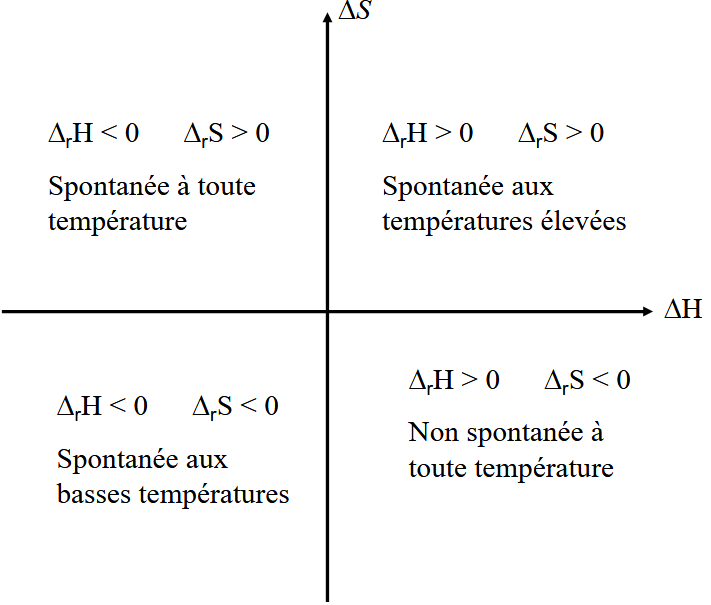
\includegraphics[scale=0.75]{./assets/temp_gibbs.png}
\caption{Effet de la température sur $\Delta_rG$}
\label{fig:temp_gibbs}
\end{center}
\end{figure}
\begin{itemize}
\item Pour $\Delta_rS$ $>$ 0 la spontanéité \textbf{augmente} quand la température augmente.
\item Pour $\Delta_rS$ $<$ 0 la spontanéité \textbf{diminue} quand la température augmente.
\end{itemize}

\chapter{L’équilibre chimique}

\section{Introduction}

\paragraph{\(\Delta_rG^0\)} Variation de G pour passer des réactifs purs aux produits purs dans des conditions standards. Au cours de la réaction, nous avons un mélange de réactifs et de produits qui change au cours du emps. \(\Delta_rG\) varie au cours de la réaction. \par
La réaction a tendance à évoluer vers le point \textbf{d’enthalpie libre minimum}.
\[\Delta_rG^0 = -RT\ln(K)\] \label{eq:GR0}
\begin{itemize}
\item \textbf{R}: constante des gaz parfaits.
\item \textbf{T}: température.
\item \textbf{K}: constante d’équilibre.
\end{itemize}
%\paragraph{La composition du mélange à l’équilibre dépend de \(\Delta_rG^0\)}
%Pour la réaction quelconque Réactifs $\rightleftarrows$ Produits à 298K.
%\begin{center}
%\begin{tabular}{| c | c | c |}
%\hline
%\textbf{\(\Delta_rG^0\) kJ$\cdot$mol$^{-1}$} & \textbf{K} & \textbf{Rapport P/R} \\
%\hline
%-9,2 & 2499 & 99,96/0,04 \\
%\hline
%-3.2 & 16 & 94/6 \\
%\hline
%-2,1 & 2,3 & 70/30 \\
%\hline
%0 & 1 & 50/50 \\
%\hline
%2,1 & 0,43 & 30/70 \\
%\hline
%3,2 & 6,4 \x 10$^{-2}$ & 6/94 \\
%\hline
%9,2 & 4 \x 10$^{-4}$ & 0,04/99,96 \\
%\hline
%\end{tabular}
%\end{center}

\section{Équilibre, quotient et constante} %TODO find a better name

\subsection{Description cinétique de l'équilibre}

Pour une réaction \textbf{réversible} de type Réactifs $\rightleftarrows$ Produits on a la notion \textbf{d'équilibre dynamique}.
\paragraph{L'équilibre dynamique} La réaction se poursuit à la même vitesse dans les 2 sens
Pas de changement macroscopique observable, la concentration de chaque réactif et produit est constante dans le temps. \par
La \textbf{constante d’équilibre K} est définie par la loi d’action de masse. Elle ne dépend pas de la composition initiale du mélange réactionnel. \\
Pour la réaction \(2R1 + R2 = 2P1\) on a K:
\[K = \frac{a_{P1}^2}{a_{R1}^2 a_{R2}}\]
Avec \textbf{a}: l'activité de l'espèce chimique\footnote{Il s'agit d'une valeur \textbf{sans unité}.}.

\subsection{Activité a$_i$ d'une espèce chimique i}

Avec \textbf{$\gamma_i$} le coefficient d'activité, $P_i$ la pression partielle de l'espèce i et $P^0$ une pression de référence\footnote{En général 1bar (100kPa) ou, si spécifié 1 atm.}, $C_i$ la concentration de l'espèce i en mol$\cdot$L$^{-1}$ et $C^0$ une concentration de référence\footnote{1 mol$\cdot$L$^{-1}$}.
\begin{itemize}
\item \textbf{Gaz}: \(a_i = \gamma_i\frac{P_i}{P^0}\), pour un gaz parfait\footnote{Valable à basse pression.} $\gamma_i$ = 1
\item \textbf{Solution diluée}: \(a_i = \gamma_i\frac{C_i}{C^0}\), dans le cas d'un solvant d'une solution \textit{très} diluée a$_{solvant}$ = 1.
\item \textbf{Solides et liquides purs}: a$_i$ = 1.
\end{itemize}
\paragraph{L'activité: une discussion} L’activité mesure essentiellement la différence entre un système réel et un système idéal. Dans le cadre de ce cours, on ne s'intéresse qu'aux systèmes idéaux, le concept d’activité n’est donc pas crucial vu que $\gamma_i$ = 1 pour tous les calculs. \par
Néanmoins, le concept d'activité permet de travailler sans unité et d'écrire correctement les constantes d'équilibres de réactions hétérogènes.

\subsection{Le quotient réactionnel Q}
Soit une réaction:
\[aA + bB \rightleftarrows cC + dD\]
\(Q = \frac{a_C^c a_D^d}{a_A^a a_B^b}\) avec les activités prises \textbf{hors de l'équilibre}. \\
\(K = \frac{a_C^c a_D^d}{a_A^a a_B^b}\) avec les activités prises \textbf{à l'équilibre}. \\
Donc on peut à partir de Q et K déduire l'évolution d'une réaction ! On peut réécrire la relation de $\Delta_rG$ en fonction de Q et K: 
\[\Delta_rG = RT\ln(\frac{Q}{K})\]
On retrouve bien $\Delta_rG$ = 0 à l'équilibre car Q = K. \\
On rappelle que $\Delta_rG^0$ s'écrit selon \ref{eq:GR0}. \\ \par
Prévision de l'évolution selon Q et K:
\begin{itemize}
\item Q $<$ K donc $\Delta_rG$ $<$ 0: Évolution vers les \textbf{produits}.
\item Q $>$ K donc $\Delta_rG$ $>$ 0: Évolution vers les \textbf{réactifs} (sens inverse).
\item Q = K donc $\Delta_rG$ = 0: Pas d'évolution, c'est \textbf{l'équilibre}.
\end{itemize}

\subsubsection{Différentes écritures de la constante K}

La constante d’équilibre peut aussi s’écrire en termes de concentration (solution) ou de
pressions partielles (gaz). Ces expressions des constantes d’équilibre sont, pour la réaction suivante: 
\[aA + bB \rightleftarrows cC\]
\(K_c = \frac{[C]^c}{[A]^a[B]^b}\) et \(K_p = \frac{(p_C)^c}{(p_A)^a(p_B)^b}\), de plus en utilisant la \ref{eq:PVNRT} on peut écrire:
\[K_c = \frac{[C]^c}{[A]^a[B]^b} = \frac{(\frac{p_C}{RT})^c}{(\frac{p_A}{RT})^a(\frac{p_B}{RT})^b} = K_p(RT)^{a+b-c}\]
De manière plus générale pour un gaz:
\[K = K_p(P^0)^{-\Delta n}\]
\[K = K_c(\frac{P^0}{RT})^{-\Delta n}\]
\[K_c = K_p(RT)^{-\Delta n}\]

\section{Équilibre et modification de l'équilibre}

\subsection{Équilibre homogène et hétérogène}

\paragraph{Équilibre homogène} Équilibre chimique dans lequel tous les réactifs et les produits sont dans la \textbf{même phase}.
\paragraph{Équilibre hétérogène} 	quilibre chimique dans lequel \textbf{plusieurs phases} sont présentes. Si des solides ou des liquides purs sont impliqués dans un équilibre, leur concentration (pression) n’apparaît \textbf{pas} dans l’expression de la constante d’équilibre de la réaction. \\
Exemple: Pour \(CaCO_3(s) \rightleftarrows CaO(s) + CO_2(g)\) on a K = a$_{CO_2}$ vu que a$_{solides}$ = 1

\subsection{Traitement qualitatif de l'équilibre}

\paragraph{Principe de Le Châtelier} Si on applique une contrainte (qui perturbe l’équilibre)
à un système en équilibre dynamique, l’équilibre tend à se déplacer dans le sens qui \textbf{minimise} l’effet de cette contrainte. \\
Les contraintes possibles sont les suivantes:
\begin{itemize}
\item Changement de la \textbf{concentration} d'un produit \textbf{ou} réactif.
\item Changement de \textbf{pression} et/ou de \textbf{volume}.
\item Changement de \textbf{température}.
\end{itemize} \par
Le principe de le Châtelier donne une appréciation \textbf{qualitative}\footnote{Qui relève de la qualité, de la nature de quelque chose (par opposition à \textbf{quantitatif}).} du changement de l'équilibre.

\subsection{Déplacements de l'équilibre}

\subsubsection{Addition ou soustraction de réactifs/produits}

Soit la réaction \(N_2(g) + 3H_2(g) \rightleftarrows 2NH_3(g)\) à l'équilibre, on a 
\[K = \frac{a_{NH3}^2}{a_{N2}\cdot a_{H2}^3}\]
\begin{itemize}
\item Si on ajoute de l'un des réactif le système est déséquilibré avec Q $<$ K donc la réaction va évoluer dans le sens \(N_2(g) + 3H_2(g) \rightarrow 2NH_3(g)\)jusqu'à atteindre un équilibre qui deviendra \textbf{le nouveau K}.
\item  Si on ajoute du produit le système est déséquilibré avec Q $>$ K donc la réaction va évoluer dans le sens \(N_2(g) + 3H_2(g) \leftarrow 2NH_3(g)\)jusqu'à atteindre un équilibre qui deviendra \textbf{le nouveau K}.
\item En résumé ajout de \textbf{réactif} = création de \textbf{produit} (déséquilibre Q $<$ K), à l'inverse ajout de \textbf{produit} = création de \textbf{réactif} (déséquilibre Q $>$ K).
\end{itemize}

\subsubsection{Compression du mélange réactionnel}

Une \textbf{compression} du système\footnote{Diminution du volume.} va entraîner un déplacement de l'équilibre de la réaction du côté permettant de \textbf{diminuer le nombre de molécules en phase gazeuse}. \\
Exemple: \(N_2(g) + 3H_2(g) \rightleftarrows 2NH_3(g)\) \par
On a 4 mol de gaz à gauche et 2 à droite, donc en cas de \textbf{compression} du système l'équilibre va se déplacer en permettant la formation de $NH_3$ car cela diminuera le nombre de moles.

\subsubsection{Variation de température}

Ajout de la chaleur provoque une évolution de l’équilibre dans le sens qui absorbe cette chaleur soit dans le \textbf{sens endothermique} de la réaction.
\begin{itemize}
\item Réaction endothermique $\Delta_rH^0$ $>$ 0 \\
Augmentation de T : réactifs + chaleur $\rightarrow$ produits
\item Réaction exothermique $\Delta_rH^0$ $<$ 0 \\
Augmentation de T : réactifs $\leftarrow$ produits + chaleur
\end{itemize} \par
Car la température modifie la constante d'équilibre \textbf{K}:
\[\ln(\frac{K_2}{K_1}) = \frac{\Delta_rH^0}{R}[\frac{1}{T_1}-\frac{1}{T_2}] \tag*{\textbf{Equation de Van’t Hoff}}\]
%TODO maybe add demo ? Slide 24 chap 5 et process de Haber-Bosch

\chapter{Cinématique Chimie}

\section{Vitesse de réaction}
À volume constant, on définit la vitesse d’une réaction chimique \textbf{v} par \textbf{la dérivée de la concentration} de l’un des produits par rapport au temps divisée par son coefficient stoechiométrique.
\[v_AA + v_BB \longrightarrow v_MM + v_NN\]

\subsection{Vitesse de consommation/production de A/M}

Exprimée en mol$\cdot$L$^{-1}$ $\cdot$s$^{-1}$:
\[v_{A/M} = \mp \frac{d[A/M]}{dt}\]
La vitesse de réaction \textbf{à volume constant}:
\[v \; = \; -\frac{1}{v_A}\frac{d[A]}{dt} =\; -\frac{1}{v_B}\frac{d[B]}{dt} = \; +\frac{1}{v_M}\frac{d[M]}{dt} \; = \; +\frac{1}{v_N}\frac{d[N]}{dt}\] 

\subsubsection{Loi de vitesse empirique}

\[v = k[A]^{\alpha}[B]^{\beta}\]
Avec
\begin{itemize}
\item v = vitesse de la réaction (mol L-1s-1)
\item k = constante de vitesse (à T const.)
\item $\alpha$ = ordre partiel en A.
\item $\beta$ = ordre partiel en B.
\item \(\alpha + \beta\) = ordre global de la réaction.
\end{itemize}
\(\alpha, \beta\): ne sont pas forcément les coefficients stochiométriques ni des nombres entiers et sont obtenus \textbf{expérimentalement}.
\paragraph{Remarque} En cinétique chimique on considère que les réactions n'ont lieu que dans \textbf{un seul sens}. Pour traiter le cas d'une réaction \textbf{bidirectionnelle} on considérera les deux réactions opposées de manière séparée.

\subsection{Réactions d'ordre X}

\subsubsection{Réactions d'ordre zéro}

Pour une réaction: \(A \longrightarrow Produits\) la loi de vitesse d'ordre 0 donne:
\[-\frac{d[A]}{dt} = k\]
\[[A](t) = [A]_0 - kt\]
Avec k $\in$ $\R$. \par
On obtient donc une diminution de la concentration à vitesse constante jusqu'à épuisement (fonction affine) qui est indépendante de la concentration des réactifs.

\subsubsection{Réactions d'ordre un}

Pour la même réaction \(A \longrightarrow Produits\) la loi de vitesse d'ordre 1 donne:
\[v = -\frac{d[A]}{dt} = k[A]\]
\[[A](t) = [A]_0e^{-kt}\]
%TODO this part is a stub on the demonstration

\subsubsection{Réactions d'ordre deux}

Pour la même réaction \(A \longrightarrow Produits\) la loi de vitesse d'ordre 2 donne:
\[v = -\frac{d[A]}{dt} = k[A]^2\]
\[\frac{1}{[A]_0} - \frac{1}{[A]_t} = -kt\]
\[\frac{1}{[A]_t} = \frac{1}{[A]_0} + kt\]

\subsection{Temps de demi-réaction}

Le temps de demi-réaction ou \textbf{demi-vie} $\tau_{1/2}$ est le temps nécessaire pour faire décroître la concentration initiale d’un réactif de moitié. \par
On a \([A]_{1/2} = \frac{1}{2}[A]_0\)

\subsubsection{Pour les réactions d'ordre un}
\[\frac{1}{2}[A]_0 = [A]_0e^{-k\tau_{1/2}}\]
\[\frac{1}{2} = e^{-k\tau_{1/2}}\]
\[\ln(\frac{1}{2}) = -k\tau_{1/2}\]
\[\frac{\ln(\frac{1}{2})}{-k} = \tau_{1/2}\]
\[\frac{0 - \ln(2)}{-k} = \tau_{1/2}\]
\begin{center}
\fbox{\(\tau_{1/2} = \frac{\ln(2)}{k}\)}
\end{center}
\par Pour les réactions du premier ordre le temps de demi-réaction ne dépend \textbf{pas} de la concentration.

\subsubsection{Pour les réactions d'ordre deux}
\[\frac{2}{[A]_0} = \frac{1}{[A]_0} + k\tau_{1/2}\]
\[\frac{1}{[A]_0} = k\tau_{1/2}\]
\[\tau_{1/2} = \frac{1}{k[A]_0}\]
\par Pour les réactions du deuxième ordre le temps de demi-réaction dépend de la \textbf{concentration initiale} du réactif.

\subsection{Résumé des ordres de réaction 0, 1, 2}\footnote{Toujours pour une réaction \(A \longrightarrow Produits\).}

\begin{figure}[h!]
\begin{center}
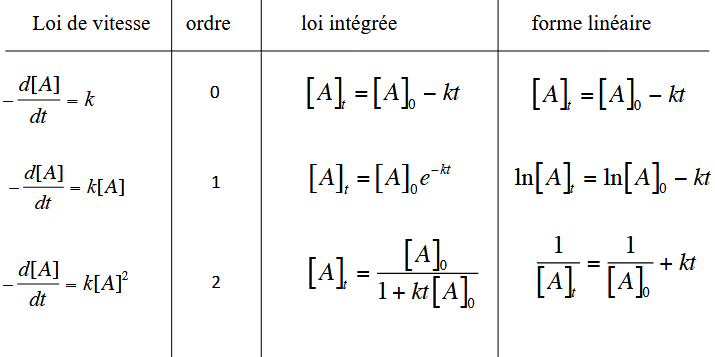
\includegraphics[scale=0.75]{./assets/reaction_order_recap.png}
\caption{Récapitulatif des ordres de réaction}
\label{fig:reaction_order_recap}
\end{center}
\end{figure}
\begin{center}
\begin{tabular}{| c | c |}
\hline
\textbf{Ordre global de réaction} & \textbf{Unité de k} \\
\hline
Zéro & \(mol\cdot L^{-1}\cdot s^{-1}\) \\
\hline
Un & \(s^{-1}\) \\
\hline
Deux & \(L\cdot mol^{-1}\cdot s^{-1}\) \\
\hline
Trois & \(L^2\cdot mol^{-2}\cdot s^{-1}\) \\
\hline
\end{tabular}
\end{center}

\subsection{Déterminer les ordres de réaction}

On peut déterminer l'ordre d'une réaction de type \(A \rightarrow Produits\) via le type de graphe ([A], ln[A], 1/[A]) en fonction de t. \par
Pour les réactions à plusieurs réactifs \(A + B + C + ... \rightarrow Produits\) on doit utiliser soit la méthode des \textbf{vitesses initiales}, soit la méthode des \textbf{réactifs en excès}.

\subsubsection{Méthode des vitesses initiales}

Soit notre réaction \(A + B + C + ... \rightarrow Produits\):
\begin{enumerate}
\item On suppose que la vitesse initiale corresponde à la vitesse moyenne au début de la réaction.
\item On définit la vitesse initiale à partir des concentrations connues des réactifs au temps t = 0.
\item On change la concentration initiale d’une seule espèce par un facteur n (connu).
\item En mesurant le rapport des vitesses de réaction on obtient l’ordre de la réaction pour l’espèce considérée.
\item On réitère le processus pour les différentes espèces chimiques.
\end{enumerate}
Soit \(v_0 = k[A]^{\alpha}_0[B]^{\beta}_0[C]^{\gamma}_0\) et \(v_0' = k[nA]^{\alpha}_0[B]^{\beta}_0[C]^{\gamma}_0\):
\[\frac{v_0'}{v_0} = \frac{k[nA]^{\alpha}_0[B]^{\beta}_0[C]^{\gamma}_0}{k[A]^{\alpha}_0[B]^{\beta}_0[C]^{\gamma}_0}\]
Si on choisit n = 2: \\
si \(\frac{v_0'}{v_0} = 1\) on aura $\alpha$ = 0. \\
si \(\frac{v_0'}{v_0} = 2\) on aura $\alpha$ = 1. \\
si \(\frac{v_0'}{v_0} = 4\) on aura $\alpha$ = 2, etc... \par
En faisant cette modification de n pour chaque espèce individuellement on peut déterminer à toutes leurs \textbf{ordres partiels}.
\\
Exemple: \(2NO(g) + Cl_2(g) \longrightarrow 2NOCl(g)\) \\
\begin{figure}[h!]
\begin{center}
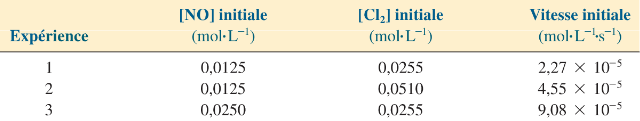
\includegraphics[scale=0.75]{./assets/method_vitesse_exemple.png}
\caption{Expériences sur les concentrations initiales}
\label{fig:speed_method_example}
\end{center}
\end{figure}
On note que la vitesse \textbf{double} pour \([nCl_2]\) avec n = 2 (expériences 1 et 2)\footnote{On fait ici référence à la figure qui suit: \ref{fig:speed_method_example}}. \\
De même on note que la vitesse \textbf{quadruple} pour \([nNO]\) avec n = 2 (expériences 1 et 3). \par
Ceci nous permet de déduire \(v = k[NO]^2[Cl_2]\)\;\;\footnote{Ici les ordres partiels correspondent aux coefficients stoechiométriques mais ce n'est \textbf{pas} un cas général.}, on peut ensuite déterminer k en introduisant les concentrations $[NO]_0$ et $[Cl_2]_0$ 

\subsubsection{Méthode des réactifs en excès}
\[n_AA + n_BB + n_CC + ... \longrightarrow Produits\]
On introduit dans ce cas là les réactifs (sauf un) en excès tel que \([A]_0 \ll [B]_0, [C]_0, ...\), ce qui nous permet de faire les approximations: \([B] \approx [B]_0\), \([C] \approx [C]_0\) et ainsi de suite.
\[-\frac{d[A]}{dt} \approx k[A]^{\alpha}[B]^{\beta}_0[C]^{\gamma}_0 = k'[A]^{\alpha}\]
Avec \(k' = k[B]^{\beta}_0[C]^{\gamma}_0\) on obtient une réaction de \textbf{pseudo-ordre $\alpha$}.
\end{document}